\ChapterImageStar[cap:dar]{Análisis de Decisiones y Resolución}{./images/fondo.png}\label{cap:dar}
\mbox{}\\

\section{Metodología de evaluación}

La metodología de evaluación aplicada para la elección de la tecnología del nuevo universo HTCondor fue \textit{Decision Analysis and Resolution} (\DAR) de \CMMI \citep{CMMIInstitute2010}. Esta metodología permitió evaluar las necesidades del grupo \GRID\ mediante un proceso estructurado que consideró múltiples alternativas, criterios de evaluación bien definidos y un análisis comparativo riguroso. Los criterios evaluados incluyeron el nivel de acoplamiento de trabajos (entendido como la capacidad de un universo para sincronizar múltiples trabajos entre sí), la capacidad de interrupción de trabajos como mecanismo para mejorar la calidad de servicio, la popularidad y adopción en el contexto académico, y la disponibilidad y calidad de documentación técnica del universo. El uso de \DAR\ no solo aporta transparencia y trazabilidad al proceso de selección, sino que también garantiza objetividad y justificación técnica sólida para la decisión arquitectónica de incorporar un nuevo universo HTCondor.

\subsection{Lista de criterios}
A continuación se describen los criterios seleccionados para la evaluación.

\subsubsection{Capacidad de paralelismo puro}
\textbf{Código:} PARALLEL

\textbf{Descripción:} Este criterio evalúa la capacidad de los diferentes universos para ejecutar computación paralela pura por medio de la comunicación entre procesos a través de algún mecanismo de \MPI como OpenMPI.

\textbf{Justificación:} En el contexto de la Universidad del Quindío es deseable para el
grupo GRID desarrollar capacidades paralelas puras en su clúster de HTCondor por
diferentes razones tales como la ejecución sincronizada y simultánea de trabajos o
la comunicación entre procesos, algunos usos de estas capacidades paralelas
pueden ser la ejecución de simulaciones distribuidas en las que la sincronización de
los trabajos es crítica debido a la ganancia temporal fruto de la comunicación en
tiempo real de los procesos, el entrenamiento paralelo de redes neuronales en el
que los pesos se actualizan de forma dinámica con la información enviada por cada
proceso paralelo, entro otros. Los casos descritos anteriormente son algunos de los
muchos en los que el soporte para trabajos paralelos puede ser deseable para el
grupo de investigación GRID, por lo que su inclusión como criterio en la toma de
decisión se considera adecuada, no como una necesidad infalible sino como un
valor adicional. Si esta fuese una necesidad infalible, entonces aquellos Universos
que no cumpliesen con capacidad para paralelismo quedarían descartados
automáticamente.

\subsubsection{Soporte para checkpointing}
\textbf{Código:} CHECKPOINTING

\textbf{Descripción:}Este criterio se refiere a la capacidad de un Universo para soportar o
no el \textit{checkpointing}. Con este término nos referimos a la capacidad de un trabajo
para ser retomado o reanudado después de su interrupción, persistiendo los valores
calculados por el proceso interrumpido hasta ese momento. Este criterio se
considera binario, ya que un Universo puede tener o no esta capacidad, cabe aclarar
que HTCondor define ciertos mecanismos de \textit{checkpointing} en su documentación
mas no aclara muy bien en cuáles Universos pueden o no ser usados, sin embargo,
es posible programar estas capacidades en capa de aplicación, lo cual se toma en
cuenta para este criterio. El único caso especial es aquel del Universo Parallel, en
el cual, según se explica en la documentación encontrada, no es posible
implementar \textit{checkpointing} debido a la naturaleza de ejecución de sus trabajos. En
los demás universos los trabajos se ejecutan de manera atómica (excepto
posiblemente el Universo Grid), es decir, de manera independiente en cada nodo,
sin embargo, la capa adicional que ofrece el \MPI en el Universo Parallel hace que
el estado actual de un trabajo no se encuentre en uno solo, sino que se encuentre
simultáneamente en todos los nodos, así como también en aquellos mensajes que
aún se encuentren en la red.


\textbf{Justificación:} La continuidad de servicio es una característica deseable para la
mayoría de las organizaciones de la industria 4.0 y el grupo GRID no es la
excepción. En este tipo de computación un nodo podría eventualmente presentar
indisponibilidad a mitad de la ejecución de un trabajo HTCondor, en este sentido el
\textit{checkpointing} se presenta como un mecanismo para evitar la pérdida de trabajo en
caso de que esto ocurra. Así pues, la capacidad para \textit{checkpointing} se considera
importante para que el grupo GRID pueda llegar a ofrecer servicios de computación
tolerantes a la variación en el estrés computacional de su infraestructura distribuida
a través de HTCondor.



\subsubsection{Popularidad}
\textbf{Código:} POPULARITY

\textbf{Descripción:} Se refiere a la cantidad de artículos, fruto del mapeo sistemático
hecho con antelación, que mencionan o indican de una u otra forma el uso o
preferencia hacia el uso de un Universo, para el problema que se aborda en los
casos de estudio propuestos por dichos artículos, para la extracción de este
criterio se realizó un proceso riguroso de estudio de mapeo sistemático en el que
se analizó parte de la literatura y se encontró la tendencia de uso de cada
Universo, al ser una medida numérica se dividió en 3 cuantiles (intervalos) de igual
tamaño y se calificó con base en qué intervalo se ubicaba cada número.


\textbf{Justificación:}Las tendencias en el uso de cada Universo en el ámbito académico
es un indicador importante de la utilidad y uso de cada Universo en ciertos casos
de estudio, a pesar de no replicar exactamente el Universo de un caso de estudio
similar, se toman casos de estudios que giran en torno a los Universos de
HTCondor, así se extraen métricas que permiten determinarlos Universos más
usados en la literatura consultada.


\subsubsection{Cantidad de documentación académica}
\textbf{Código:} DOC

\textbf{Descripción:} Se refiere a la documentación académica encontrada en torno a
este Universo, específicamente en el motor de búsqueda “Google Scholar”. Este
criterio difiere de la popularidad, ya que se usa un método menos exhaustivo para
su medición, además, en el criterio popularidad solo se toman en cuenta los casos
de estudio en bases de datos específicas, por el contrario, en este caso se hace
una medición general en un motor de búsqueda ampliamente usado. Esta medida
toma relevancia cuando se considera el hecho de que pueden haber Universos
muy populares pero poco documentados, y en tal caso, dichos universos podrían
no ser idóneos para la implementación en la infraestructura HTCondor del GRID.


\textbf{Justificación:} La cantidad de documentación disponible respecto a cierto
Universo hace más sencilla la correcta documentación de la arquitectura
propuesta para la infraestructura del GRID, esto cobra relevancia cuando
consideramos que la poca documentación es uno de los problemas hallados en
el diagrama de Ishikawa realizado en torno a las debilidades y problemáticas que
existen alrededor de la infraestructura HTCondor de GRID y debe ser mitigado
para que ayude a la mitigación del efecto general.

\subsubsection{División de roles}
\textbf{Código:} ROLE DIV

\textbf{Descripción:} Este criterio toma en cuenta la división de roles por máquina.
Esencialmente, los clústeres HTCondor convencionales tienen tres roles: Central
Manager, Submit Node y Execute. En un entorno ideal estos roles deben estar
separados en diferentes máquinas, sin embargo, existen Universos en los que
estos roles no se dividen en varias máquinas y son ejecutados por un solo nodo
de cómputo, lo que no se alinea con las causas que se quieren mitigar.

\textbf{Justificación:} La división de trabajos es una situación deseable para la
infraestructura HTCondor del GRID, ya que así cada nodo de cómputo tendrá una
única responsabilidad y se evitará sobrecargar un equipo con múltiples funciones
lo que propende por una administración atómica al mismo tiempo que aumenta la
facilidad e implementación mecanismos de recuperación y redundancia a cada
rol.



\subsection{Lista de Universos de HTCondor}
Tras definir los criterios, se identificaron los Universos disponibles en la tecnología HTCondor \citep{HTCondor-choosing-universe}:
\begin{itemize}
	\item vanilla
	\item grid
	\item java
	\item scheduler
	\item local
	\item parallel
	\item vm
	\item container
	\item docker
\end{itemize}

\subsection{Medición de la popularidad}
El criterio de ``popularidad'' se definió como el volumen de uso de un Universo en artículos científicos, por lo que se requirió un proceso metódico para su medición. Para ello, se procedió con un estudio de mapeo sistemático \SMS (ver sección \ref{cap:revisionLiteratura}). El SMS es un método definido para analizar literatura existente, extrayendo recursos de varias fuentes y seleccionándolos con criterios rigurosos. El resultado final es una taxonomía que permite contar las apariciones de cada Universo en la literatura seleccionada.

El proceso completo es robusto e incluye múltiples etapas; sin embargo, para fines de este documento, lo más relevante es el diagrama del proceso (Figura \ref{fig:sms}) y los resultados obtenidos (Tabla \ref{tab:aparicion_universos}).


\begin{figure}[H]
	\centering
	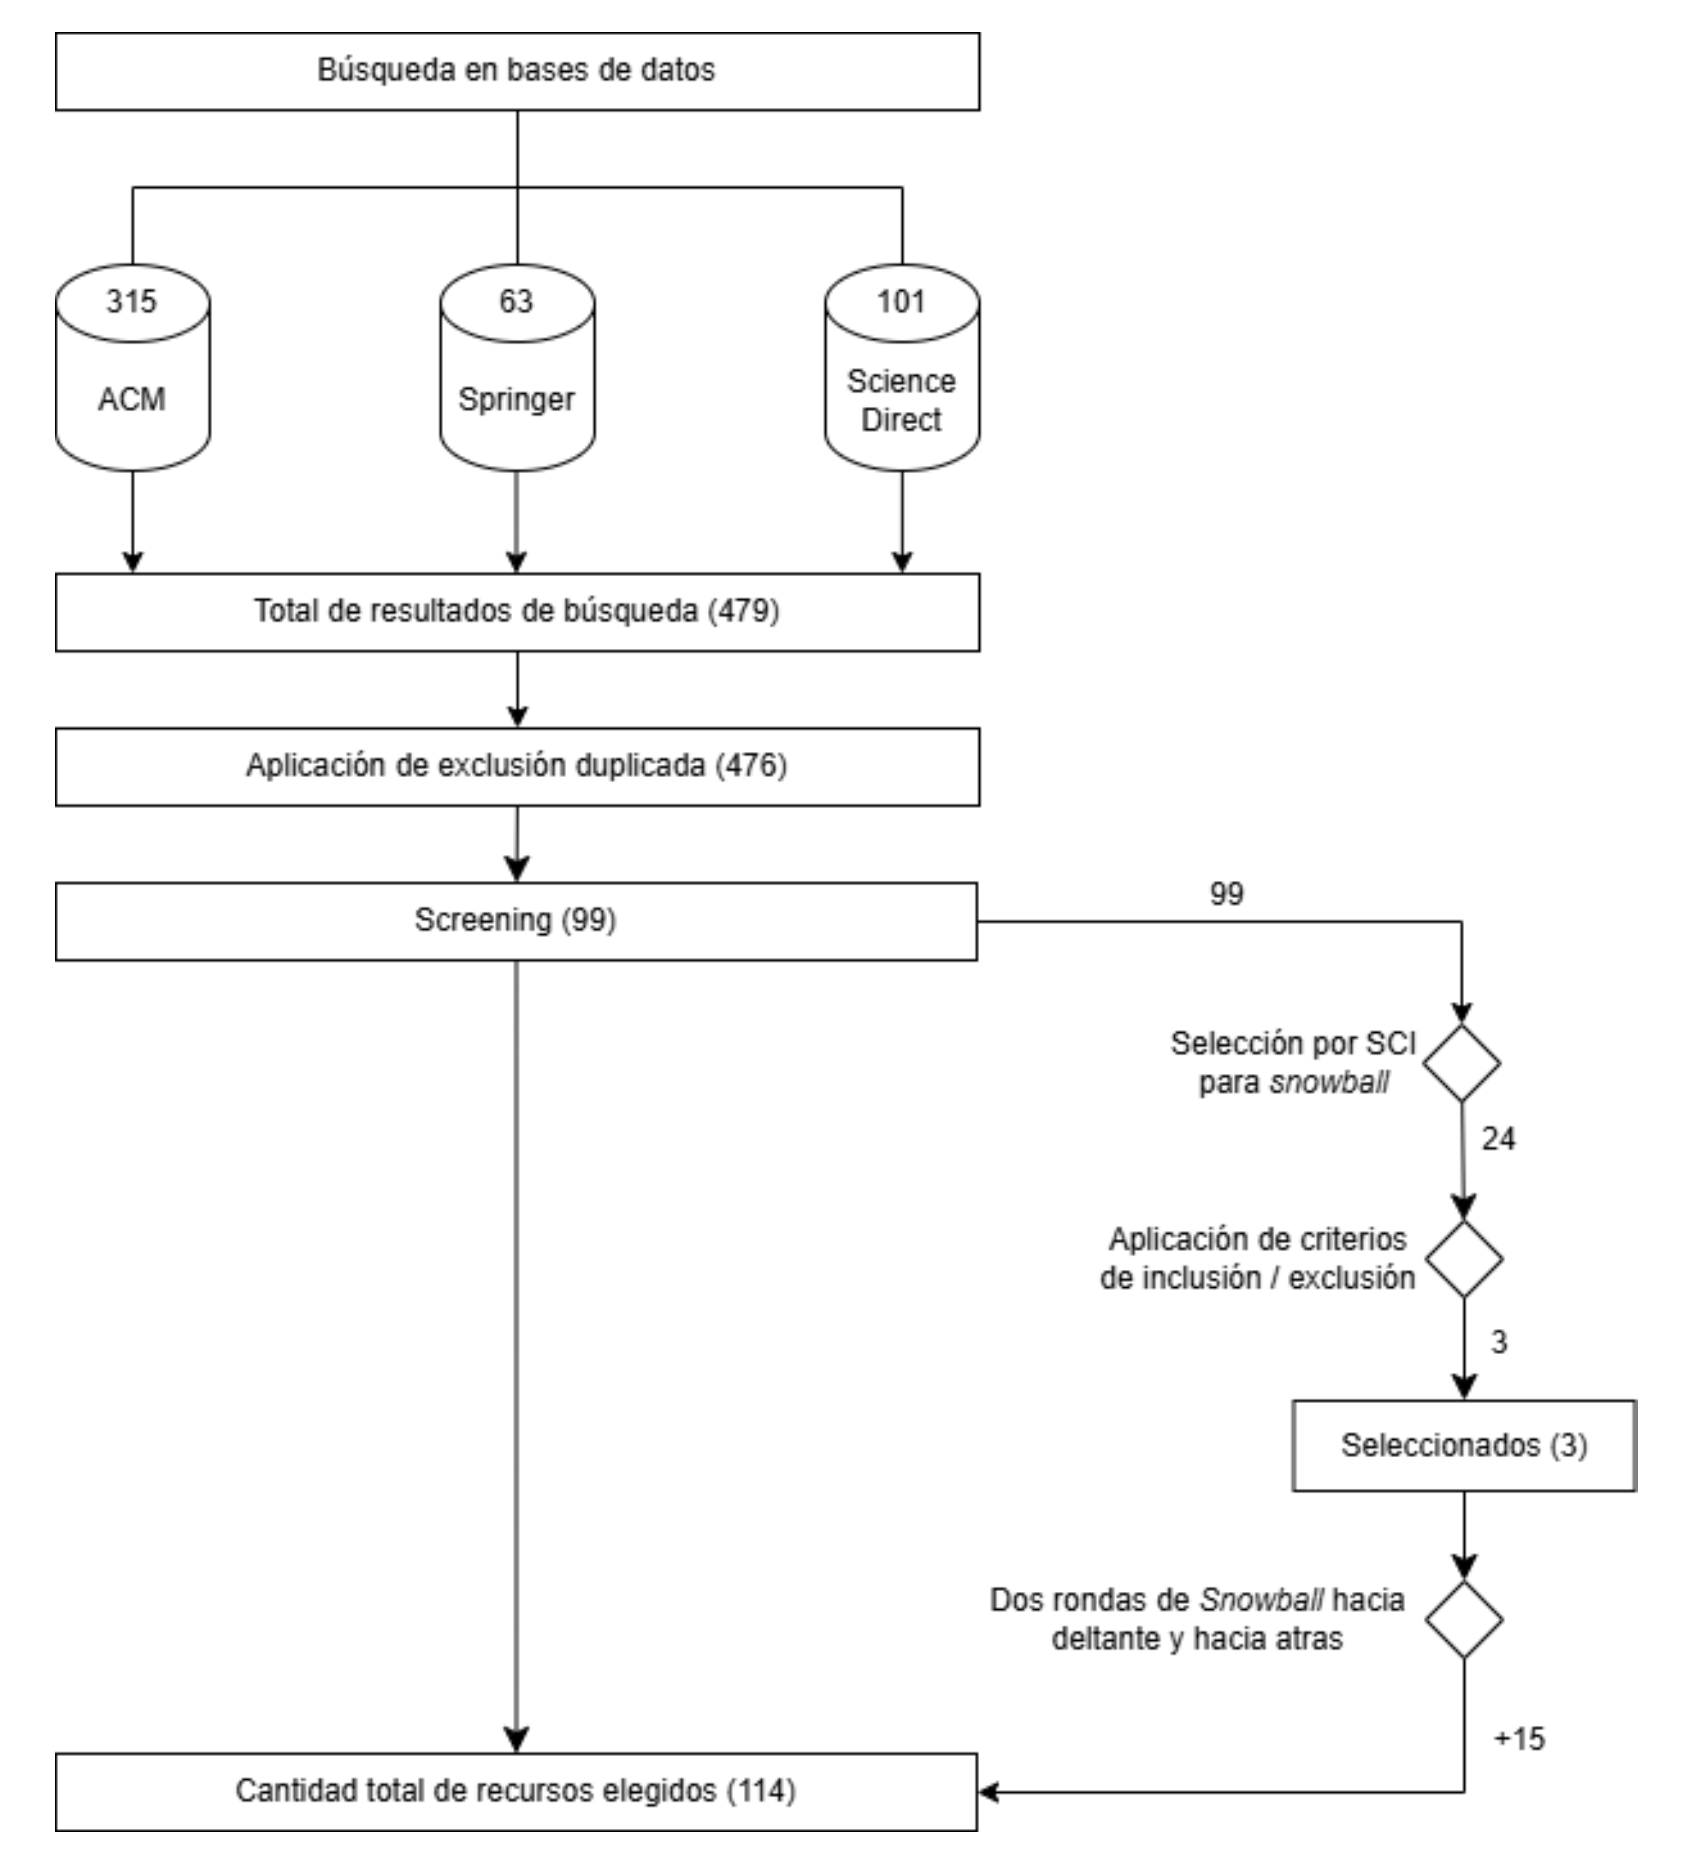
\includegraphics[scale=0.4]{tablas-images/dar/resumen-mapeo.png}
	\caption{Estudio de mapeo sistemático (\SMS).}
	\label{fig:sms}
\end{figure}

La Tabla \ref{tab:aparicion_universos} muestra los resultados del mapeo, donde la primera columna indica el universo, la segunda los códigos de los artículos relacionados con dicho universo, y la tercera el conteo total de artículos por Universo.

\begin{table}[H]
	\centering
	\renewcommand{\arraystretch}{1.2} % Espaciado reducido
	\fontsize{9pt}{10pt}\selectfont % Tamaño de fuente 8pt
	\caption{Aparición de universos en la literatura.}
	\label{tab:aparicion_universos}
	\begin{tabular}{|l|p{8cm}|c|}
		\hline
		\textbf{Universo} & \textbf{SPS ID (Estudios)}                                                                                                                                                                                                                                                                                                                                                                       & \textbf{Suma por Universo} \\
		\hline
		Parallel          & \tiny{SPS006 SPS007 SPS009 SPS010 SPS013 SPS017 SPS021 SPS024 SPS025 SPS026 SPS032 SPS034 SPS035 SPS037 SPS038 SPS041 SPS042 SPS043 SPS044 SPS045 SPS046 SPS049 SPS050 SPS054 SPS061 SPS065 SPS066 SPS068 SPS070 SPS071 SPS072 SPS073 SPS074 SPS075 SPS077 SPS079 SPS080 SPS082 SPS083 SPS084 SPS085 SPS092 SPS093 SPS094 SPS096 SPS101 SPS103 SPS104 SPS105 SPS106 SPS109 SPS110 SPS111 SPS112} & 54                         \\
		\hline
		Vanilla           & \tiny{SPS016 SPS017 SPS018 SPS020 SPS027 SPS028 SPS029 SPS031 SPS032 SPS033 SPS039 SPS044 SPS045 SPS047 SPS049 SPS050 SPS058 SPS063 SPS067 SPS070 SPS076 SPS078 SPS080 SPS086 SPS087 SPS088 SPS089 SPS090 SPS095 SPS097 SPS099 SPS102 SPS108 SPS109 SPS111 SPS113 SPS103}                                                                                                                        & 37                         \\
		\hline
		Container         & \tiny{SPS004 SPS011 SPS019 SPS025 SPS026 SPS034 SPS035 SPS037 SPS038 SPS044 SPS053 SPS080 SPS081 SPS084 SPS085 SPS108}                                                                                                                                                                                                                                                                           & 16                         \\
		\hline
		Grid              & \tiny{SPS001 SPS002 SPS003 SPS005 SPS006 SPS008 SPS009 SPS014 SPS015 SPS017 SPS018 SPS028 SPS029 SPS040 SPS046 SPS048 SPS052 SPS053 SPS055 SPS057 SPS060 SPS061 SPS062 SPS064 SPS065 SPS066 SPS069 SPS074 SPS075 SPS087 SPS089 SPS090 SPS091 SPS092 SPS098 SPS100 SPS107 SPS112 SPS114}                                                                                                          & 39                         \\
		\hline
		Docker            & \tiny{SPS004 SPS019 SPS036 SPS053 SPS085}                                                                                                                                                                                                                                                                                                                                                        & 5                          \\
		\hline
		Java              & \tiny{SPS043}                                                                                                                                                                                                                                                                                                                                                                                    & 1                          \\
		\hline
	\end{tabular}
\end{table}

\subsection{Análisis DAR}
Con los criterios definidos y la medición de popularidad completada, se procedió a realizar el análisis DAR, cuyos resultados se presentan en la Tabla \ref{tab:analisis_dar}.

\begin{table}[H]
	\centering
	\renewcommand{\arraystretch}{1.2} % Espaciado reducido
	\fontsize{9pt}{10pt}\selectfont % Tamaño de fuente 8pt
	\caption{Análisis DAR.}
	\label{tab:analisis_dar}
	\begin{tabular}{|>{\centering\arraybackslash}p{2.0cm}|>{\centering\arraybackslash}p{1.5cm}|>{\centering\arraybackslash}p{2.5cm}|>{\centering\arraybackslash}p{2.1cm}|>{\centering\arraybackslash}p{0.8cm}|>{\centering\arraybackslash}p{1.8cm}|>{\centering\arraybackslash}p{1.6cm}|}
		\hline
		{\scriptsize\textbf{Criterio}} & {\tiny\textbf{PARALLEL}}                           & {\tiny\textbf{CHECKPOINTING}}  & {\tiny\textbf{POPULARITY}} & {\tiny\textbf{DOC}} & {\tiny\textbf{ROLE DIV}} & {\tiny\textbf{}} \\
		\hline
		{\scriptsize\textbf{UNIVERSO}} & \multicolumn{5}{c|}{{\scriptsize\textbf{Puntaje}}} & {\scriptsize\textbf{Promedio}}                                                                                                  \\
		\hline
		Vanilla                        & 1                                                  & 3                              & 3                          & 3                   & 3                        & 2,6              \\
		\hline
		Grid                           & 2                                                  & 3                              & 3                          & 2                   & 3                        & 2,6              \\
		\hline
		Java                           & 1                                                  & 3                              & 1                          & 1                   & 3                        & 1,8              \\
		\hline
		Scheduler                      & 1                                                  & 3                              & 1                          & 1                   & 3                        & 1,8              \\
		\hline
		Local                          & 1                                                  & 3                              & 1                          & 1                   & 1                        & 1,4              \\
		\hline
		Parallel                       & 3                                                  & 1                              & 3                          & 3                   & 3                        & 2,6              \\
		\hline
		VM                             & 1                                                  & 3                              & 3                          & 1                   & 3                        & 2,2              \\
		\hline
		Container                      & 1                                                  & 3                              & 1                          & 1                   & 3                        & 1,8              \\
		\hline
		Docker                         & 1                                                  & 3                              & 1                          & 1                   & 3                        & 1,8              \\
		\hline
	\end{tabular}
	\vspace{5pt}
\end{table}

\section{Resultados y Pasos Futuros}

\subsection{Resumen del análisis}
El proceso ejecutado tuvo como fin tomar una decisión informada sobre el Universo a implementar en la infraestructura HTCondor del GRID. Considerando el resultado descrito en la Tabla \ref{tab:analisis_dar}, hubo un empate en los Universos ganadores Grid y Parallel. Teniendo en cuenta esta situación que no se tenía en cuenta desde el principio, se tomó la decisión de continuar con las demás etapas del proyecto con ambos Universos, ya que no hay motivos, razones ni evidencia para orientarnos por uno o por otro.

Grosso modo, el Universo Grid funciona como un middleware o intermediario que hace de puente para enviar trabajos computacionales desde un nodo submit hacia un pool HTCondor de recursos externos. Por su parte, el Universo Parallel ejecuta programas que hacen usos de alguna implementación de MPI (Message Passing Interface) como OpenMPI para lograr así una ejecución sincronizada y ordenada para permitir la comunicación entre los nodos.

\subsection{Próximos pasos}
Se procederá con el diseño de las arquitecturas de la solución con cada Universo y su posterior implementación a través de un prototipo funcional.
